\documentclass[12pt, a4paper]{article}
\usepackage[utf8]{inputenc}
\usepackage{amsmath}
\usepackage{amsthm}
\usepackage{graphicx}
\usepackage{parskip}
\usepackage{hyperref}
\usepackage{fancyhdr}
\usepackage{lastpage}
\usepackage{tikz}
\usepackage{float}
\usepackage[acronym]{glossaries}

\tikzstyle{bag} = [align=center]

\title{%
      Homework 1 \\
      Experimental Prove of $\theta(\log n)$ height on Random Binary Search Trees
}
\author{Juan Pablo Royo Sales}
\date\today

\pagestyle{fancy}
\fancyhf{}
\fancyhead[C]{}
\fancyhead[R]{Juan Pablo Royo Sales - UPC MIRI}
\fancyhead[L]{ADS - Homework 1}
\fancyfoot[L,C]{}
\fancyfoot[R]{Page \thepage{} of \pageref{LastPage}}
\setlength{\headheight}{15pt}
\renewcommand{\headrulewidth}{0.4pt}
\renewcommand{\footrulewidth}{0.4pt}

\makeglossaries

\newacronym{bst}{BST}{Binary Search Tree}
\newacronym{rbst}{RandomBST}{Randomly Built Binary Search Tree}
\newacronym{treap}{Treap}{Treap}
\newacronym{rtreap}{RTreap}{Randomized Treap}

\begin{document}

\maketitle

\section{Introduction}
In this Homework I have selected to explore and analyze \textbf{\acrfull{rbst}} in order to prove through experimentation that the expected height of \textit{\acrshort{rbst}} is $E[h] = \theta(\log n)$ as it is formally proved in \cite{cormen}.

In order to do that we are going to first give a brief introduction to this type of Data Structure and the theoretical analysis of this feature.

\section{Randomly Built Binary Search Tree}
A \acrshort{rbst} is a \textbf{\acrfull{bst}} that is specifically built using random insertions, in order to achieve \textbf{balanced} \acrshort{bst} \textit{whp}.

Given an insertion in a \acrshort{rbst} of size $n - 1$ there exists the same probability for the key to be inserted in the same interval that the keys already present in the tree. Basically all $n{!}$ possible permutations of the keys are equally likely.

There exists a specific implementation, which is the one I used to conduct the analysis, which is \textbf{\acrfull{rtreap}}.

In the following sections I am going to describe this Data Structure that fulfill the specification of an \acrshort{rbst}.

\section{Treap and Randomized Treap}
A \textbf{\acrfull{treap}} is a \acrshort{bst} in which every node has both the proper key and a priority associated with it $(k_i, p_i)$, such that the Left subtree $L$ of an specific node $N_i = (k_i, p_i)$ contains keys which priorities are less than the parent $\forall j, j \in L \land j \neq i \implies k_i \geq k_j \land p_i \geq p_j$. On the other hand the right subtree $R$ of $N_i$ contains the greater keys and priorities such that $\forall j, j \in R \land j \neq i \implies k_i \leq k_j \land p_i \leq p_R$. A \acrshort{treap} can be seen as a \acrshort{bst} for the search keys and a min-heap for the priorities.

\begin{figure}[H]
\centering
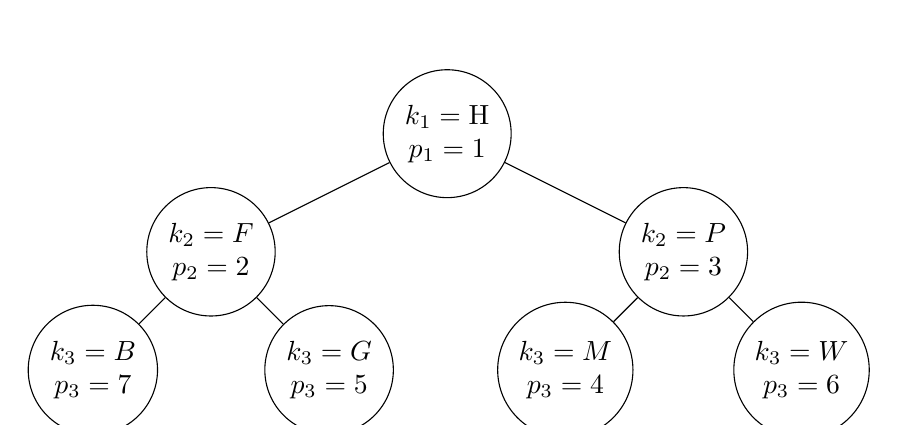
\begin{tikzpicture}[level/.style={sibling distance=60mm/#1}]
  \node [bag,circle,draw](z){
    $k_1 = \text{H}$ \\
    $p_1 = 1$}
    child {node [bag,circle,draw] (a) {$k_2 = F$ \\ $p_2 = 2$}
      child {node [bag,circle,draw] (d) {$k_3 = B$ \\ $p_3 = 7$}}
      child {node [bag,circle,draw] (e) {$k_3 = G$ \\ $p_3 = 5$}}
    }
    child {node [bag,circle,draw] (a) {$k_2 = P$ \\ $p_2 = 3$}
      child {node [bag,circle,draw] (d) {$k_3 = M$ \\ $p_3 = 4$}}
      child {node [bag,circle,draw] (e) {$k_3 = W$ \\ $p_3 = 6$}}
    };
\end{tikzpicture}
\caption{Treap Example} \label{fig:treap_fig_ex}
\end{figure}

\printglossary[type=\acronymtype]

\begin{thebibliography}{9}
\bibitem{cormen}
  Cormen, T.H., Stein, C., Rivest, R.L., Leiserson, C.E. 2001. \textit{Introduction to Algorithms}. 2nd edn. McGraw-Hill Higher Education.
\end{thebibliography}


\end{document}

